\input ../preamble

\begin{document}

{\Huge

  \centerline{\bf TTIC 31230, Fundamentals of Deep Learning}
  \bigskip
  \centerline{David McAllester, Winter 2018}
  \vfill
  \centerline{\bf Language Modeling}
  \vfill
  \centerline{\bf Machine Translation}
  \vfill
  \centerline{\bf Attention}
  \vfill
  \centerline{\bf Beam Search}
  \vfill
  \centerline{\bf Error-Based Training}
  

\slide{Language Modeling}

We are given a sequence $x^1$, $\ldots$, $x^T$ and we want to compute a model probability.

\vfill
$$Q_\Phi(x_1,\ldots,x^T)$$

\vfill
Here $x^t$ can be either characters or words.

\vfill
We represent the probability as a product of conditionals.

\vfill
$$Q_\Phi(x_1,\ldots,x^T) = \prod_t Q_\Phi(x^t \;|\; x^1,\ldots,x^{t-1})$$

\vfill
A model of this form is called {\bf Autoregressive} --- a model (regression) is used to predict the next element from the previous elements.

\slide{RNN Language Modeling}

\centerline{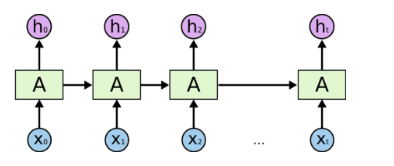
\includegraphics[width=3.5in]{../images/RNN}}
\centerline{{\large [Christopher Olah]}}

$$Q_\Phi(x^{t+1} \;|\; x^1,\ldots,x^t) = \mathrm{Softmax}(W^o\;h^t)$$

\vfill
For word language models this softmax is the computation bottleneck in training.

\slide{Standard Measures of Performance}

{\bf Bits per Character:}
For character language models performance is measured in bits per character.  Typical numbers are slightly over one bit per character.

\vfill
{\bf Perplexity:}
It would be natural to measure word language models in bits per word.  However, it is traditional to measure then in perplexity which is defined to be
$2^b$ where $b$ is bits per world.  Perplexities of about 60 are typical.

\vfill
According to Quora there are 4.79 letters per word.  1 bit per character (including space characters) gives a perplexity of $2^{5.79}$ or $55.3$.

\slide{Sampling From an Autoregressive Model}

To sample a sentence
\vfill
$$x^1,\ldots, x^T, \mbox{\tt <eos>}$$
\vfill
we sample $x^t$ from
\vfill
$$Q_\Phi(x^t|x^1,\ldots,x^{t-1})$$

\vfill
until we get {\tt <eos>}.

\anaslide{Machine Translation}

\centerline{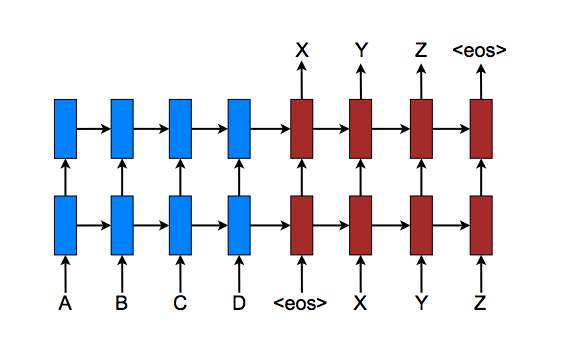
\includegraphics[width = 4in]{../images/SeqToSeq}}

\centerline{\large [Figure from Luong et al.]}

$$DCBA \Rightarrow XYX$$

\vfill
Translation is a {\bf sequence to sequence} (seq2seq) task.

\vfill
{\bf Sequence to Sequence Learning with Neural Networks}, Sutskever, Vinyals and Le, NIPS 2014, arXiv Sept 10, 2014.

\anaslideplain{Machine Translation}

\centerline{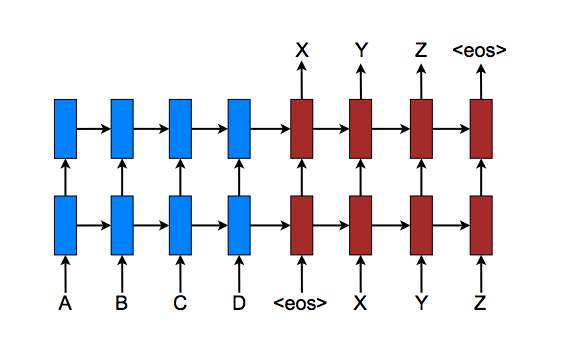
\includegraphics[width = 4in]{../images/SeqToSeq}}

\centerline{\large [Figure from Luong et al.]}

\vfill
The input sentence is represented by a ``thought vector'' produced by an RNN.

\anaslide{Machine Translation}

\centerline{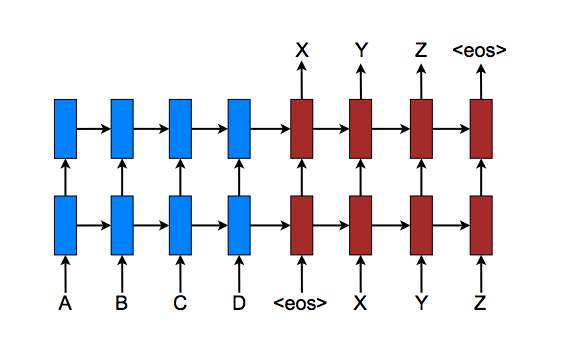
\includegraphics[width = 4in]{../images/SeqToSeq}}

\centerline{\large [Figure from Luong et al.]}

\vfill
The thought vector is the initial state vector used in ``sampling'' a translation.

\anaslide{Machine Translation}

\centerline{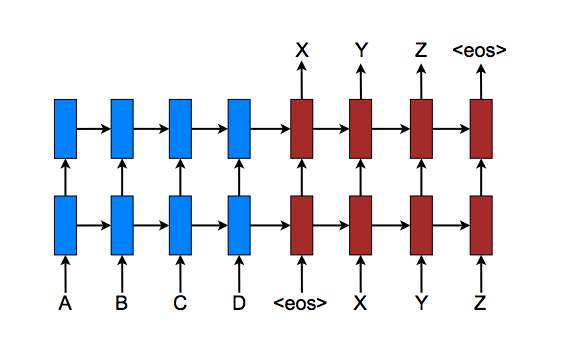
\includegraphics[width = 4in]{../images/SeqToSeq}}

\centerline{\large [Figure from Luong et al.]}

\vfill
For the training pair $DCBA \Rightarrow XYX$ the training loss is

\vfill
$$- \log\;Q_\Phi(XYZ\;|\;DCBA)$$


\anaslide{Machine Translation}

\centerline{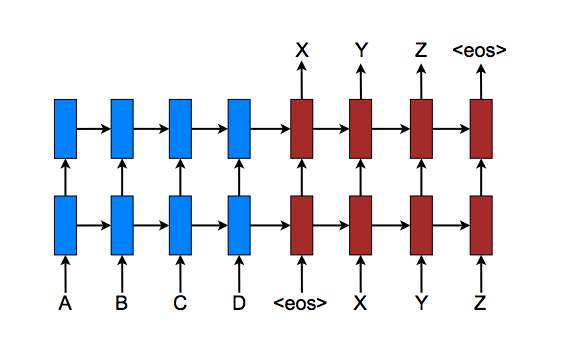
\includegraphics[width = 4in]{../images/SeqToSeq}}

\centerline{\large [Figure from Luong et al.]}

\vfill
In Sutskever et al. (2014) the LSTMs are layered 4 deep.

\ignore{
\slide{Training Details (Sutskever et al. (2014))}

We used deep LSTMs with 4 layers, with 1000 cells at each layer and 1000 dimensional word embeddings, with an input vocabulary
of 160,000 and an output vocabulary of 80,000.

\vfill
We used a naive softmax over 80,000 words at each output.

\vfill
We used batches of 128 sequences.

\vfill
We used stochastic gradient descent without momentum, with a fixed learning rate of 0.7.

\vfill
After 5 epochs, we begun halving the learning rate every half epoch. We trained our models
for a total of 7.5 epochs.

\slide{Training Details}

[We clipped gradients] by scaling [the gradient] when its norm exceeded 5.

\vfill
Different sentences have different lengths. ... To address this problem, we made
sure that all sentences within a minibatch were roughly of the same length. [This gave] a 2x
speedup.

\slide{Training Details}

We parallelized our [C++] model using an 8-GPU machine.

\vfill
Each layer of the LSTM was executed on a different GPU and communicated its activations to the next GPU (or layer) as soon
as they were computed.

\vfill
Our models have 4 layers of LSTMs, each of which resides on a separate
GPU.

\centerline{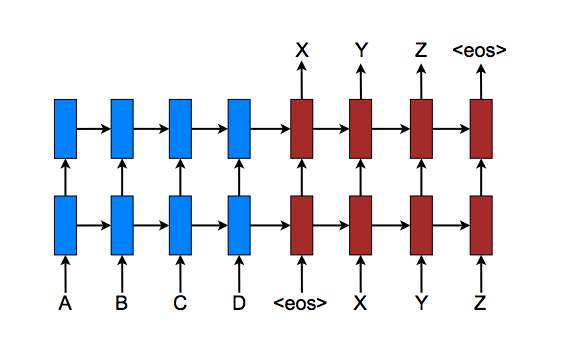
\includegraphics[width = 4.0in]{../images/SeqToSeq}}

\slide{Training Details}

\vfill
The remaining 4 GPUs were used to parallelize the softmax, so each GPU was responsible
for multiplying by a 1000 × 20,000 matrix. [20,000 is 1/4 of the output vocabulary]

\vfill
Training took about ten days with this implementation [on a training set of 348M French words and 304M English words].
}

\slide{Attention-Based Translation}

Translation is improved by aligning input words with output words.

\vfill
This is done with ``Attention''.

\vfill
{\bf Neural Machine Translation by Jointly Learning to Align and Translate}
Dzmitry Bahdanau, Kyunghyun Cho, Yoshua Bengio, ICLR 2015 (arXiv Sept. 1, 2014)

\slide{Attention}

The input sentence is no longer represented by just one thought vector.

\vfill
Instead the entire sequence of hidden vectors produced by the RNN is used during generation of the translation.

\slide{Attention}

\centerline{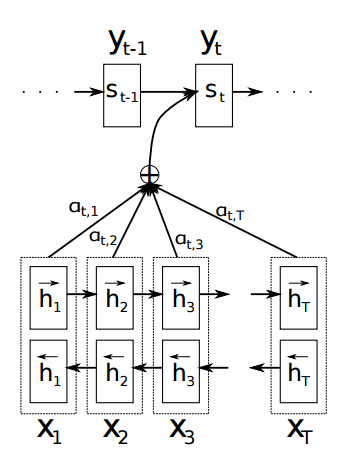
\includegraphics[height=4.5in]{../images/attention}}
\centerline{[Bahdanau, Cho, Bengio (2014)]}

\slide{A first step: BiRNNs}

\begin{eqnarray*}
  \vec{h}^{t+1} & =  & \mathrm{RNNCELL}_\Phi(\vec{h}^t,x^t) \\
  \\
  \\
  \cev{h}^{t-1} & =  & \mathrm{RNNCELL}_\Psi(\cev{h}^t,x^t) \\
  \\
  \\
  \dvec{h}^t & = & \left[\vec{h}^t,\cev{h}^t\right]\;\;\;\;\;\;\left([x,y]\;\mbox{denotes vector concatenation}\right)
\end{eqnarray*}

\vfill
\anaslide{Basic Sequence to Sequence Model}

\begin{eqnarray*}
  \\
  s^0 & = & \vec{h}^T \\
  y^0 & = & <\!\!\mathrm{eos}\!\!> \\
  \\
  Q^\Phi(:\;| {\bf x},\;y^1,\ldots,y^i) & = & \softmax_{\hat{y}} \;W^y \;s^{i+1}\;\;\;\;\;\;\;\;\mbox{~} \\
  s^{i+1} & = & \mathrm{RNNCELL}_\Phi(s^i,\;e(y^i)))
\end{eqnarray*}

\anaslide{Adding Attention}

\begin{eqnarray*}
  {\color{red} c^0} & = & \dvec{h}^T \\
  s^0 & = & \vec{h}^T \\
  y^0 & = & <\!\!\mathrm{eos}\!\!> \\
  \\
  Q_\Phi(:\;| {\bf x},\;y^1,\ldots,y^i) & = & \softmax_{\hat{y}} \;W^y \;s^{i+1} \\
  s^{i+1} & = & \mathrm{RNNCELL}_\Phi(s^i,\;[e(y^i),\;{\color{red} c^i}]) \\
  \\
  {\color{red} c^i} & = & \sum_t {\color{red} \alpha^{i,t}} \dvec{h}^t  \\
  {\color{red} \alpha^{i,t}} & = & \softmax_t\; \mathrm{tanh}(W^a\;[s^i,\;\dvec{h}^t])
\end{eqnarray*}

\slideplain{Attention}

\centerline{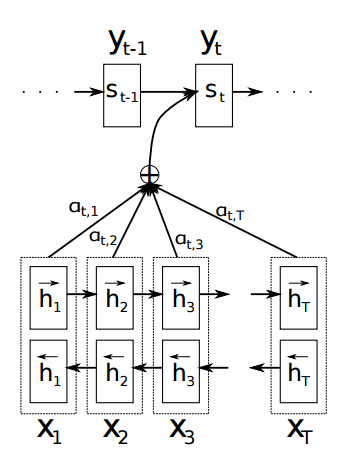
\includegraphics[height=4.5in]{../images/attention}}
\centerline{[Bahdanau, Cho, Bengio (2014)]}

\anaslide{Bilinear Attention is More Popular Today}

\begin{eqnarray*}
  {\color{red} c^0} & = & \dvec{h}^T \\
  s^0 & = & \vec{h}^T \\
  y^0 & = & <\!\!\mathrm{eos}\!\!> \\
  \\
  Q_\Phi(:\;| {\bf x},\;y^1,\ldots,y^i) & = & \softmax_{\hat{y}} \;W^y \;s^{i+1} \\
  s^{i+1} & = & \mathrm{RNNCELL}_\Phi(s^i,\;[e(y^i),\;{\color{red} c^i}]) \\
  \\
  {\color{red} c^i} & = & \sum^t {\color{red} \alpha^{i,t}} \dvec{h}^t  \\
  {\color{red} \alpha^{i,t}} & = & \softmax_t\; {\color{red} (s^i)^\top W^a \dvec{h}^t}
\end{eqnarray*}

\slideplain{Attention in Image Captioning}

\centerline{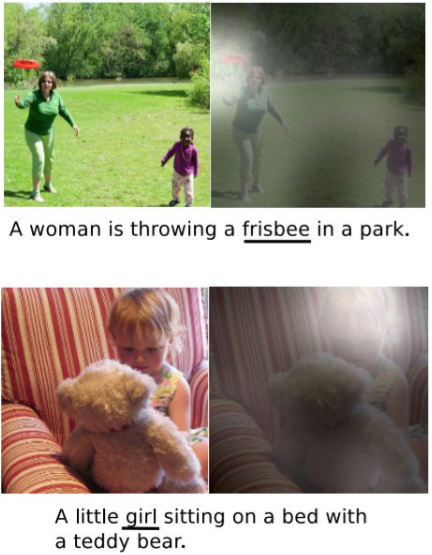
\includegraphics[width = 4in]{../images/AttentionInCaptioning1}}
\centerline{Xu et al. ICML 2015}

\slide{Greedy Decoding vs. Beam Search}

We would like

\vfill
$${\bf y}^* = \argmax_{\bf y} Q_\Phi({\bf y}|{\bf x})$$

\vfill
A {\bf greedy algorithm} may do well

\vfill
$$y^{t+1} = \argmax_{\hat{y}}\; Q_\Phi(\hat{y}\;|\;{\bf x},\;y^1,\ldots,y^t)$$

\vfill
But these are not the same.

\slide{Example}

$${\bf y}^* = \argmax_{\bf y} Q_\Phi({\bf y}|{\bf x})$$

$$y^{t+1} = \argmax_{\hat{y}}\; Q_\Phi(\hat{y}\;|\;{\bf x},\;y^1,\ldots,y^t)$$

\vfill
\vfill
``Those apples are good'' vs. ``Apples are good''

\vfill
$$Q_\Phi(\mbox{Apples are Good {\tt <eos>}}) > Q_\Phi(\mbox{Those apples are good {\tt <eos>}})$$

\vfill
$$Q_\Phi(\mbox{Those}|\varepsilon) > Q_\Phi(\mbox{Apples}|\varepsilon)$$
    
\slide{Beam Search}

At each time step we maintain a list of $k$ word-vector pairs:

\vfill
\begin{eqnarray*}
  Y^t & = & ((y^{t,1},h^{t,1}),\ldots,(y^{t,k},h^{t,k}) \\
  \\
  \\
  Y^{t+1} & = & \kbest_{(\hat{y},\hat{h})\in C^t} \; Q_\Phi(y\; |\; {\bf x},\;Y^1,\ldots,Y^t) \\
  \\
  \\
  C^t & = & \left\{(y^{t+1,i,j},h^{t+1,i}):\;\;\begin{array}{rcl}
  y^{t+1,i,j} & \in & \kbest_{\hat{y}}\;Q_\Phi(\hat{y}|(y^{t,i},h^{t,i})) \\
  \\
  h^{t+1,i,j} & = & \mathrm{RNNCELL}(h^{t,i},e(y^{t,i,j}))
  \end{array}\right\}
  \end{eqnarray*}

\slideplain{Error-Based Training}

Systems are often evaluated by error rather than loss (log loss).

\vfill
Should we train directly to minimize error?

\vfill
Should translation be trained directly on BLEU score?

\vfill
Should segmentation be trained on intersection over union?

\vfill
Should cancer screening be trained on  recall?

\vfill
If the model provides probabilities we can do Bayesian inference.  But the model might not be sufficiently expressive.

\anaslide{Label Adjustment}
We can consider an arbitrary error function $\mathrm{Err}(y,\hat{y})$ assigning an error value the true label is $y$ and the system guesses $\hat{y}$.

\begin{eqnarray*}
  f(\hat{y}) & = & \sum_\alpha\; f[\alpha,\hat{y}[\alpha]] \\
  \\
  \hat{y}^*(f) & = & \argmax_{\hat{y}} \; f(\hat{y}) \\
  \\
  \breve{y}^*(f) & = & \argmax_{\breve{y}} \;f(\breve{y}) - \epsilon \mathrm{Err}(y,\breve{y}) \;\;\;\;\mbox{\bf (adjusted label)} \\
  \\
  \mathrm{error}(y,f) & = & \mathrm{Err}(y,\hat{y}^*(f)) \\
  \\
  f_\Phi(x).\mathrm{grad}[\alpha,\tilde{y}] & \minuseq & \eta\left(\mathbbm{1}[\hat{y}^*_{f_\Phi(x)}[\alpha] = \tilde{y}]
  - \mathbbm{1}[\breve{y}^*_{f_\Phi(x)}[\alpha] = \tilde{y}]\right) 
\end{eqnarray*}

\anaslideplain{Label Adjustment Theorem}
\begin{eqnarray*}
    f_\Phi(x).\mathrm{grad}[\alpha,\tilde{y}] & \minuseq & \eta\left(\mathbbm{1}[\hat{y}^*_{f_\Phi(x)}[\alpha] = \tilde{y}]
  - \mathbbm{1}[\breve{y}^*_{f_\Phi(x)}[\alpha] = \tilde{y}]\right) 
\end{eqnarray*}

\vfill
{\bf Theorem}: For a continuous and smooth population distribution
\begin{eqnarray*}
  & & \nabla_\Phi  \;E_{(x,y) \sim \mathrm{Pop}}\;\mathrm{Err}(y,\hat{y}^*(f_\Phi(x))) \\
  \\
  & = & \lim_{\epsilon \rightarrow 0} \;\frac{1}{\epsilon}\; E_{(x,y) \sim \mathrm{Pop}} \\
  \\
  & & \;\;\;\;\;\;\sum_{\alpha,\tilde{y}} \left(\;\mathbbm{1}[\hat{y}^*_{f_\Phi(x)}[\alpha] = \tilde{y}]
  - \mathbbm{1}[\breve{y}^*_{f_\Phi(x)}[\alpha] = \tilde{y}] \right) \nabla_\Phi f_\Phi(x)[\alpha,\tilde{y}]
\end{eqnarray*}



\slide{Intersection over Union}

In visual detection problems one is typically evaluated by {\bf intersection over union}.

$$\mathbf{IOU} = \frac{|\mbox{true positives} \cap \mbox{false positives}|}{|\mbox{true positives} \cup\mbox{false positives}|} = \frac{P - FN}{P + FP}$$

\vfill
\begin{eqnarray*}
    \frac{\partial \mathrm{}IOU}{\partial \mathrm{FP}} & =  & \frac{-(P - FN)}{(P + FP)^2} = \frac{-\mathrm{IOU}}{P+ FP} \\
    \\ \\
    \frac{\partial \mathrm{}IOU}{\partial \mathrm{FN}} & =  & \frac{-1}{P + FP}
\end{eqnarray*}

\slideplain{Phrase Based Statistical Machine Translation (SMT)}

Step I:   Learn a phrase table --- a set of triples $(p,q,s)$ where

\vfill
\begin{itemize}
\item $p$ is a (short) sequence of source words.
  \vfill
\item $q$ is a (short) sequence of target words.
  \vfill
\item $s$ is a score.
\end{itemize}

\vfill
(``au'', ``to the'', .5) \hfill (``au banque'', ``the the bank'', .01)

\vfill
For a phrase $P$ we will write $P.\mathrm{source}$ for the source phrase, $P.\mathrm{target}$ for the target phrase, and $P.\mathrm{score}$ for the score.

\slide{Derivations}

Consider an input sentence $x$ of length $T$.

\vfill
We will write $x[s:t]$ for the substring $x[s]$, $\ldots$, $x[t-1]$.

\vfill
A derivation $d$ from $x$ is a sequence $(P_1,s_1,t_1,)$, $\ldots$, $(P_K,s_K,t_K)$ where $P_k.\mathrm{source} = x[s_k:t_k]$.

\vfill
The substrings $x[s_k:t_k]$ should be disjoint and ``cover'' $x$.

\vfill
For $d = [(P_1,s_1,t_1,)$, $\ldots$, $(P_L,s_K,t_K)]$ we define

$$ y(d) \equiv P_1.\mathrm{target}\;\cdots P_K.\mathrm{target}$$

\vfill
We let $D(x)$ be the set of derivations from $x$.

\slide{Scoring}

For $d \in D(x)$ we define a score $s(d)$

\vfill
$$s(d) = \alpha \ln P_\mathrm{LM}(y(d)) + \beta \sum_k P_k.\mathrm{score} + \gamma \;\mathrm{distortion}(d)$$

\vfill
where $P_{\mathrm{LM}}(y)$ is the probability assigned to string $y$ under a language model for the target language

\vfill
and $\mathrm{distortion}(d)$ is a measure of consistency of word ordering between source and target strings as defined by
the indeces $(s_1,t_1)$, $\ldots$, $(s_K,t_K)$.

\slide{Translation}

\begin{eqnarray*}
  y(x) & = & y(d^*(x)) \\
  \\
  \\
  \\
  d^*(x) & = & \argmax_{d \in D(x)} \;s(d)
\end{eqnarray*}

\slide{END}
\end{document}
